%! Suppress = LabelConvention
\setboolean{@twoside}{false}

\section*{Appendix A: Paper}
\label{app:paper}
This paper was been produced with the authors being myself, Dr Sebastian Stein, Professor Tim Norman from Southampton
University, Dr Fidan Mehmeti, Professor Tom La Porta, Caroline Rubein from Pennsylvania State University and Dr Geeth
Demel from IBM and within this project is referred to as~\cite{FlexibleResourceAllocation}.

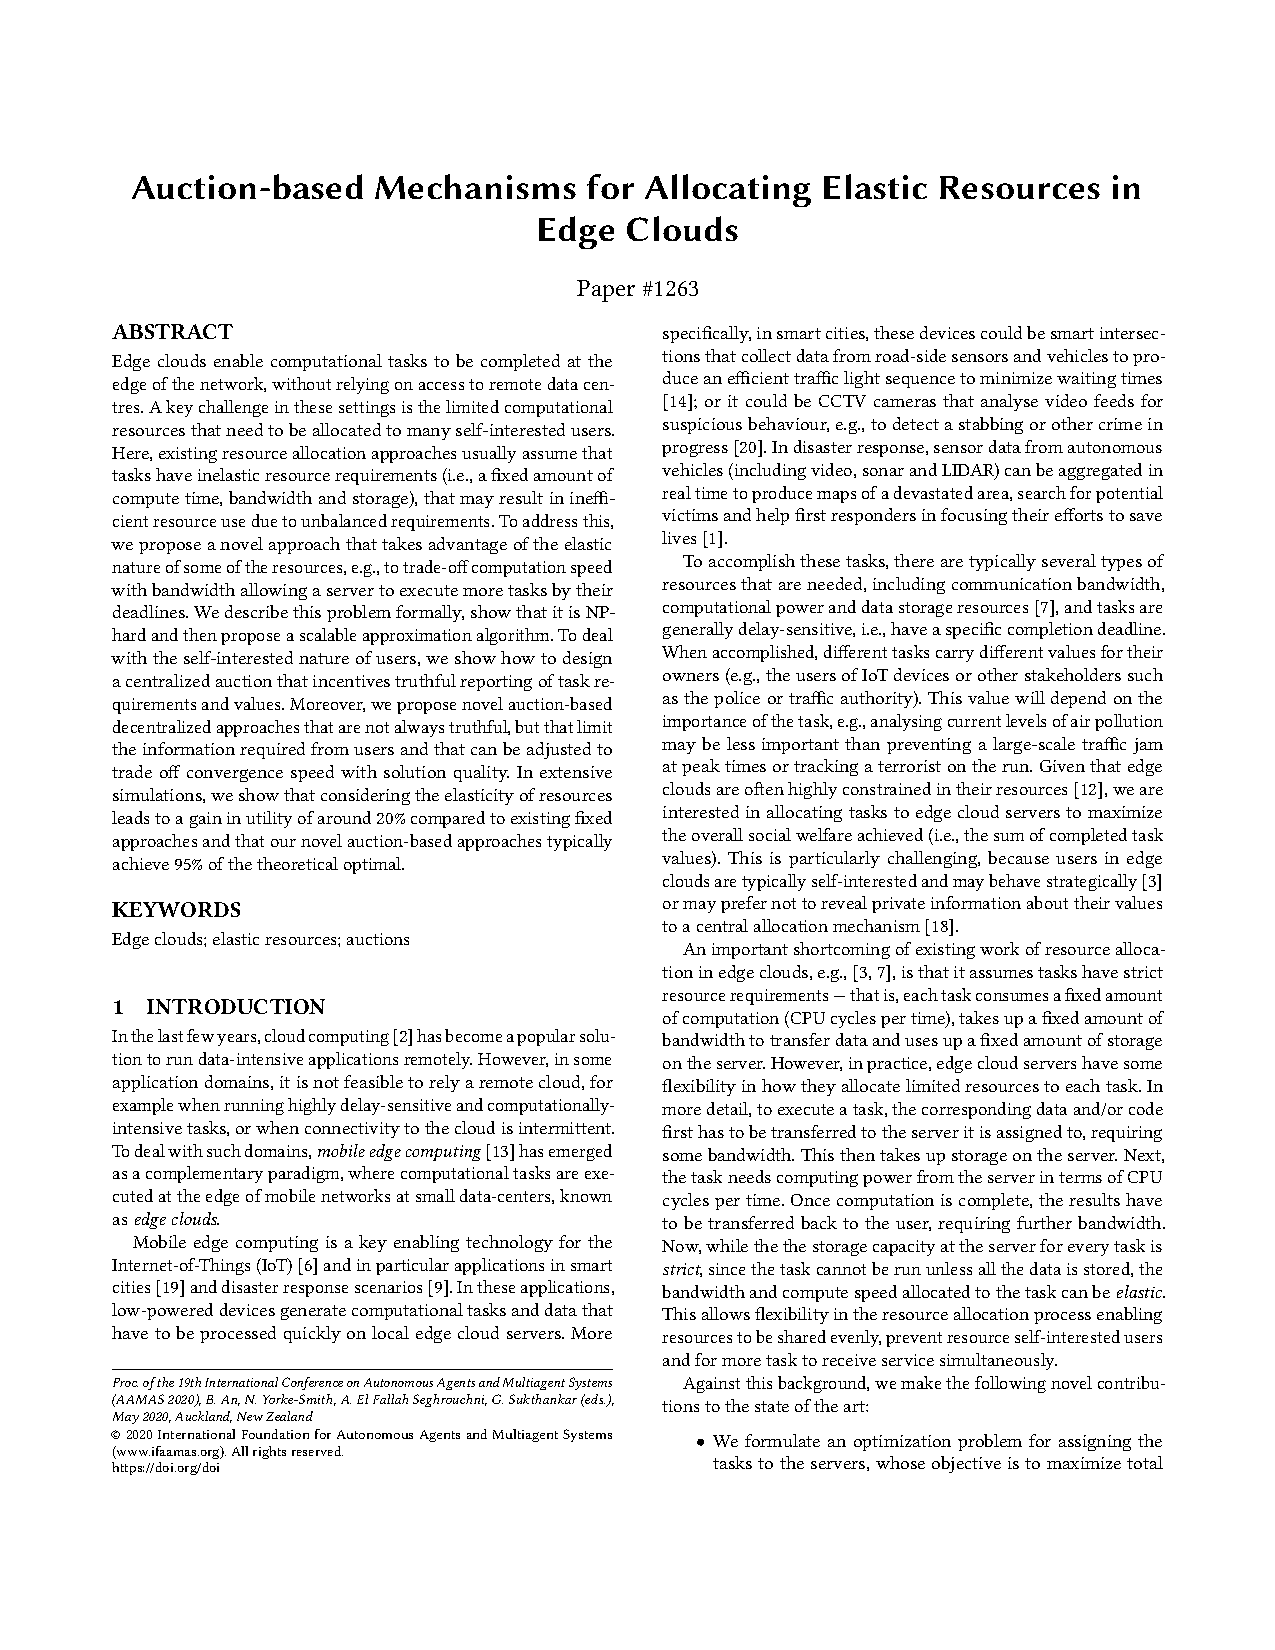
\includepdf[pages=-, offset=25mm -20mm]{extra/aamas_2020}

\section*{Appendix B: SPIE Presentation}
\label{app:spie-presentation}
The research of~\cite{FlexibleResourceAllocation} was presented at SPIE Defense + Commercial Sensing to the conference
on Artificial Intelligence and Machine Learning for Multi-Domain Operations Applications II under the title
"Analytical agility at the edge of the network through auction mechanisms".
\href{https://spie.org/SI/conferencedetails/artificial-intelligence-and-machine-learning-for-multi-domain-battle-applications#2560056}{Link}
to the recorded presentation.

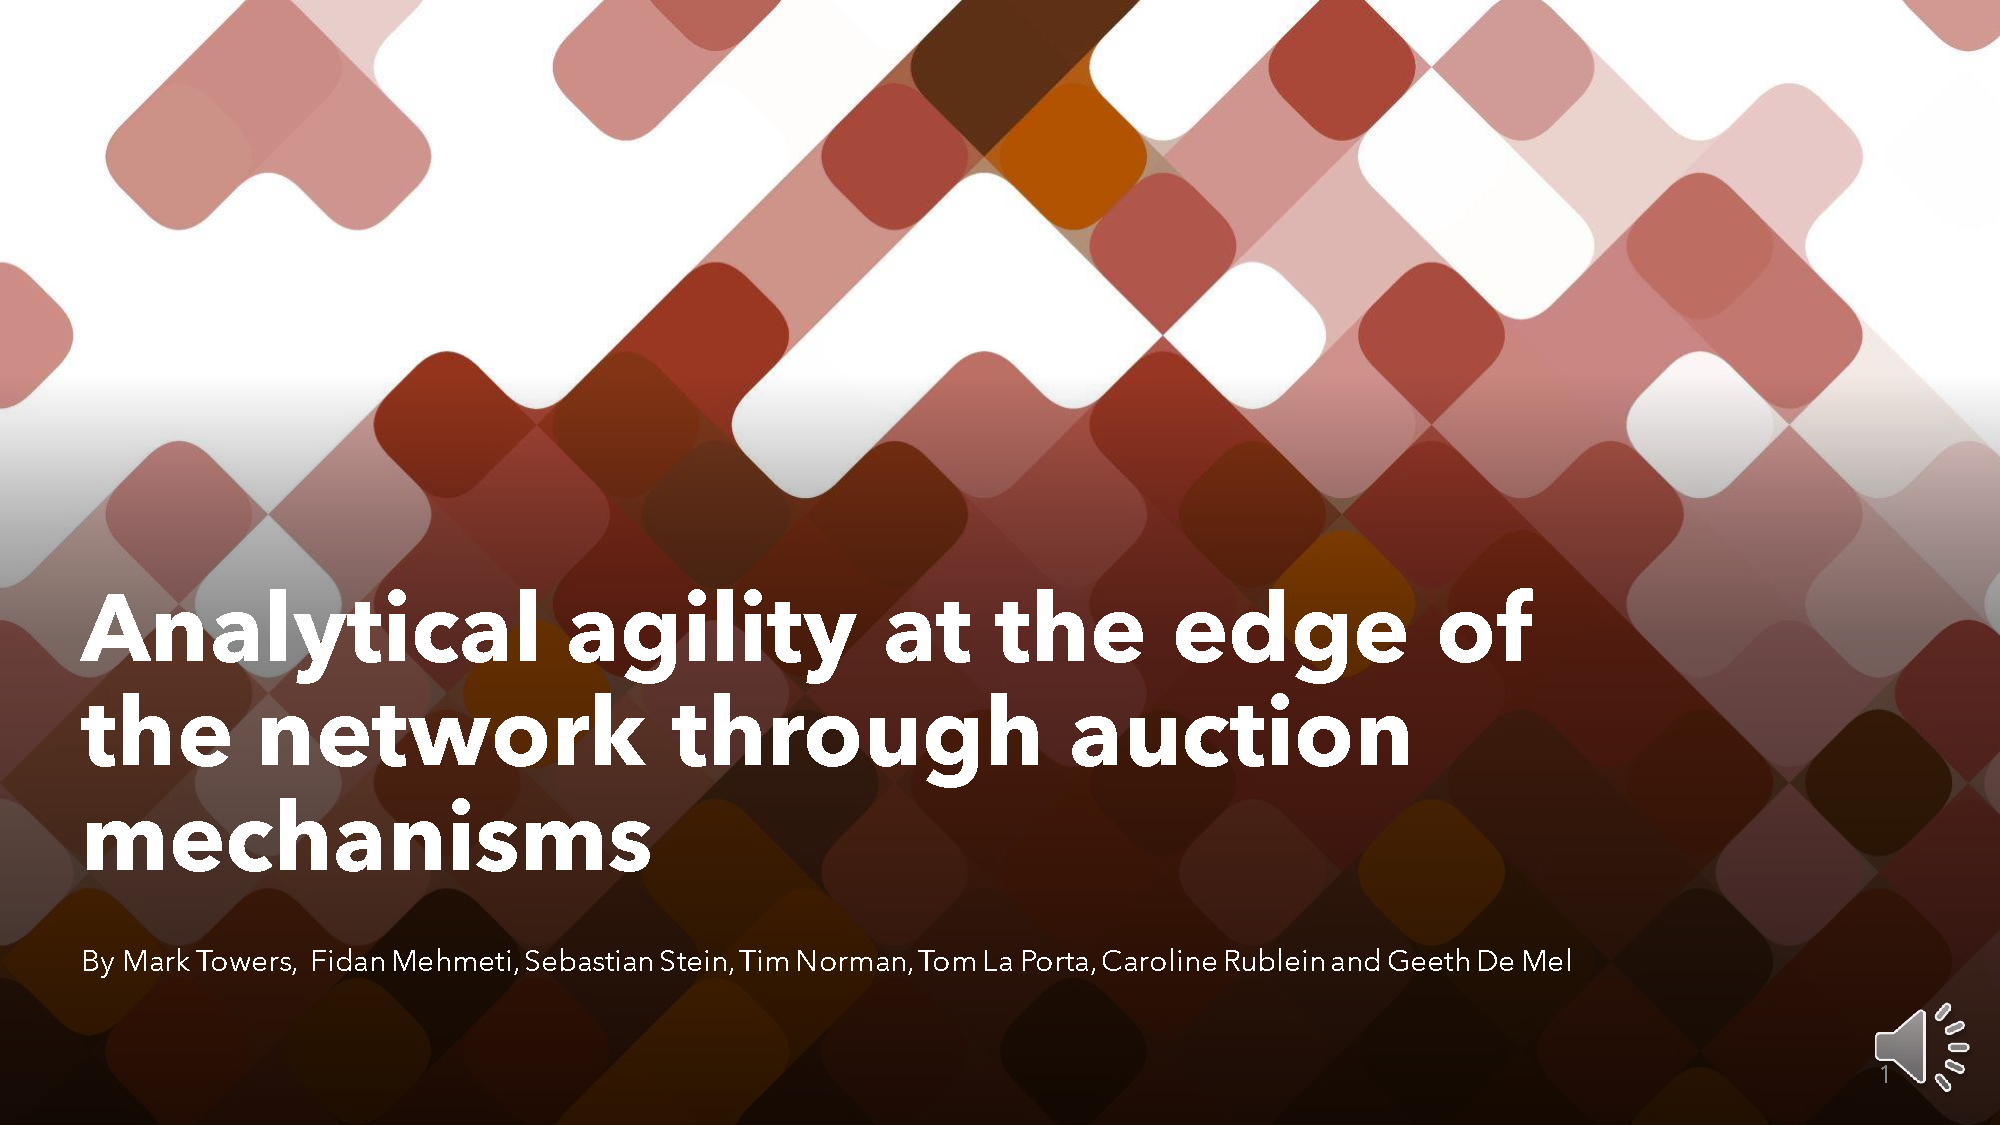
\includepdf[pages=-, offset=25mm -25mm, landscape=True, scale=0.95]{extra/spie_presentation}

\section*{Appendix C: Agent hyperparameters}
\label{app:agent-hyperparameters}
During training there are a range of hyperparameters for each agent, table~\ref{tab:agent_hyperparameters} provides
an explanation for the values for each hyperparameter used in the project.

\begin{longtable}{|p{2cm}|p{3.5cm}|p{2.5cm}|p{6cm}|} \hline
    \textbf{Agent} & \textbf{Properties name} & \textbf{Value} & \textbf{Explanation} \\ \hline
        RL Agent & batch\_size & 32 & The number of trajectories from the experience replay buffer that are used each
            time to train an agent. \\ \hline
        RL Agent & error\_loss\_fn & tf.losses. huber\_loss & The loss function used in calculating a network's error. \\ \hline
        RL Agent & initial\_training\_ replay\_size & 5000 & The number of trajectories in the experience replay buffer
            required before the agent begins training. \\ \hline
        RL Agent & training\_freq & 2 & For every trajectory added to the experience replay buffer, for each 2, the
            agent tries to be trained. \\ \hline
        RL Agent & discount\_factor & 0.9 & Within the Q learning function (equation~\eqref{eq:q_learning}), the
            discount factor determines how important the rewards in the future impact the Q value. \\ \hline
        RL Agent & replay\_buffer\_ length & 25000 & The length of the circular experience replay buffer. \\ \hline
        RL Agent & save\_frequency & 25000 & The agent networks are saved after 25000 time that agent has been trained
            \\ \hline
        RL Agent & training\_loss\_ log\_freq & 250 & Tensorboard allows for data to be saved using training, after every
            the agent has been trained 250 time, the agents loss is logged for future analysis. \\ \hline
        Task Pricing RL Agent & reward\_scaling & 1 & \\ \hline
        Task Pricing RL Agent & failed\_auction\_ reward & -0.05 & The reward for when the agent bids on a task but fails
            to win the auctioned task. \\ \hline
        Task Pricing RL Agent & failed\_multiplier & -1.5 & A multiplier applied to the winning price is the task fails
            to be computed within its deadline. \\ \hline
        Resource weighting RL Agent & other\_task\_discount & 0.4 & The multiplier to tasks not under consideration for
            a weighting action. \\ \hline
        Resource weighting RL Agent & success\_reward & 1 & The reward when the agent successfully completes a task
            \\ \hline
        Resource weighting RL Agent & failed\_reward & -1.5 & The reward when the agent fails to complete a task within
            its deadline. \\ \hline
        Dqn Agent & target\_update\_tau & 1.0 & The update tau value for use in the target update frequency. \\ \hline
        Dqn Agent & target\_update\_freq & 2500 & The target network in the DQN agent is updated after the agent
            has been updated 2500 times. \\ \hline
        Dqn Agent & initial\_epsilon & 1 & The initial exploration factor during training \\ \hline
        Dqn Agent & final\_epsilon & 0.1 & The final exploration factor during training \\ \hline
        Dqn Agent & epsilon\_steps & 10000 & The number of training step for linear exploration to move between the
            initial\_epsilon and the final\_epsilon factor. \\ \hline
        Dueling Dqn Agent & double\_loss & True & If to use the double dqn loss function \\ \hline
        Categorical Dqn Agent & max\_value & -20.0 & The maximum value for the value distribution \\ \hline
        Categorical Dqn Agent & min\_value & 25.0 & The minimum value for the value distribution \\ \hline
        Categorical Dqn Agent & num\_atoms & 21 & The number of atoms for each actions. \\ \hline
        Ddpg Agent & actor\_learning\_rate & 0.0001 & The learning rate for the optimiser for the actor network. \\ \hline
        Ddpg Agent & critic\_learning\_rate & 0.0005 & The learning rate for the optimiser for the critic network. \\ \hline
        Ddpg Agent & initial\_epsilon\_std & 0.8 & The initial exploration standard deviation of the normal distribution
            used  during training \\ \hline
        Ddpg Agent & final\_epsilon\_std & 0.05 & The final exploration standard deviation of the normal distribution
            used  during training \\ \hline
        Ddpg Agent & actor\_target\_ update\_freq & 3000 & The actor target network update frequency \\ \hline
        Ddpg Agent & critic\_target\_ update\_freq & 1500 & The critic target network update frequency \\ \hline
        Ddpg Agent & upper\_action\_ bound & 30.0 & The upper action bound for the actor network \\ \hline
        Task pricing Ddpg Agent & min\_value & -100.0 & The minimum value for the critic network to estimate for an
            action \\ \hline
        Task pricing Ddpg Agent & max\_value & 100.0 & The maximum value for the critic network to estimate for an
            action\\ \hline
        Resource allocation Ddpg Agent & min\_value & -20 & The minimum value for the critic network to estimate for an
            action \\ \hline
        Resource allocation Ddpg Agent & max\_value & 15 & The maximum value for the critic network to estimate for an
            action\\ \hline
        TD3 Agent & actor\_update\_freq & 3 & The actor network update frequency for each critic network update. \\ \hline
    \caption{Agent hyperparameters}
    \label{tab:agent_hyperparameters}
\end{longtable}

\section*{Appendix D: Fixed Resource Allocation Optimisation Problem}
\label{app:fixed-resource-allocation-optimisation-problem}
Using the Flexible Resource Allocation Optimisation problem from Section~\ref{sec:resource-allocation-optimisation-problem},
to convert the problem to a Fixed Resource Allocation Optimisation problem requires two stages. \\
The first of these is to convert the flexible task specification to a fixed task specification, by solving the linear
programming equations~\ref{eq:fixed-task-objective} and~\ref{eq:fixed-task-deadline}. The equations forces the resource
usage speeds ($s^{'}_j$, $w^{'}_j$ and $r^{'}_j$) to be within the deadline (equation~\ref{eq:fixed-task-deadline}) and
that the objective function is to minimise the total resources used. The reason for speeds being raise to the power is
to prevent over use of a single resources (e.g. 5 loading speeds, 3 compute speed, 10 sending speed).

\begin{align}
    \text{minimise  } & 1.2^{s^{'}_j} + 1.2^{w^{'}_j} + 1.2^{r^{'}_j} \label{eq:fixed-task-objective} \\
    \mbox{s.t.} \nonumber \\
    & \frac{s_j}{s^{'}_j} + \frac{w_j}{w^{'}_j} + \frac{r_j}{r^{'}_j} \leq d_j - a_j \label{eq:fixed-task-deadline} \\
\end{align}

The second stage is using the Fixed task specifications, to construct the server resource allocation optimisation
problem. The objective function (equation~\ref{eq:fixed-env-objective}) is to maximise the number of tasks that are
completed. The updated fixed tasks are denoted $J^{'}$. Due to there being a fixed resource allocation, the server
allocates all of the required resources over the tasks whole lifetime. As a result, the server computational and
bandwidth capacity constraints (equations~\ref{eq:fixed-server-computation-capacity}
and~\ref{eq:fixed-server-bandwidth-capacity}) allocates a task's resources over its whole lifetime. The server's storage
constraint is similar except with a task's storage increasing till the whole task's required storage is included.

\begin{align}
    \text{max} & \sum_{i \in I, j \in J^{'}} x_{i,j} \label{eq:fixed-env-objective} \\
    \mbox{s.t.} \nonumber \\
    & \sum_{\{j \in J^{'} | a_j \leq t \leq d_j\}} \text{min}(s_j \text{, } s^{'}_j \cdot (t + 1 - a_j)) \cdot x_{i,j} \leq S_i && \forall{i \in I} \label{eq:fixed-server-storage-capacity} \\
    & \sum_{\{j \in J^{'} | a_j \leq t \leq d_j\}} w^{'}_j x_{i,j} \leq W_i && \forall{i \in I} \label{eq:fixed-server-computation-capacity} \\
    & \sum_{\{j \in J^{'} | a_j \leq t \leq d_j\}} (s^{'}_j + r^{'}_j) \cdot x_{i,j} \leq R_i && \forall{i \in I} \label{eq:fixed-server-bandwidth-capacity} \\
    & \sum_{i \in I} x_{i,j} \leq 1 && \forall{j \in J^{'}} \label{eq:fixed-env-allocation-limit} \\
    & x_{i,j} \in \{0, 1\} && \forall{i \in I, j \in J^{'}} \label{eq:fixed-env-allocation-set}
\end{align}

\section*{Appendix E: Project management}
\label{app:project-management}
To management this project has been difficult due to splitting my time between writing the academic paper at the
start of the year (plus creating the recorded presentation) and the programming and write up the expanded research.
Because of this, a risk assessment (Table~\ref{tab:risk_assessment}) to understand possible risks during the project.
The project was also planned using a grantt chart (figure~\ref{fig:progress-grant-chart}) to understand the progress of
the project over time and to plan how the project would run. The project brief is submitted in October 2019
is included at the end of this report as well. The word count of the project generated by texcount for chapters 1 to 6
is included.

The general plan for the project in the project briefing was kept to with very small changed like the real-world data
from the Google data center was found to be incompatible with the resource requirements therefore dropped.

\subsection*{Risk assessment}
\begin{table}[H]
    \centering
    \begin{tabular}{|p{3cm}|c|c|p{7cm}|} \hline
        \textbf{Risk}  & \textbf{Severity} & \textbf{Possibility} & \textbf{Explanation} \\ \hline
        Rejected paper submission & 1 & 4 & The paper (Appendix A) was submitted to the AAMAS 2020 conference in
            December that could be rejected. While this was be disappointing if this happened, the paper can still be
            submitted to another conference at a later time. \\ \hline
        Iridis failure & 5 & 1 & In order to train the agent in this project, the University of Southampton supercomputer,
            Iridis 5 was utilised so if this could not be used anymore. This was cause massive issues to be able to
            train all of the agents for both long enough. \\ \hline
        Agent Training time & 4 & 2 & Reinforcement learning agents can take several million actions to achieve
            effective results which takes days or weeks to learn. This project doesn't have such resources or time to
            spend training agents to do this therefore making it a large problem. \\ \hline
        Personal Illness or Injury & 4 & 1 & Physical illness or injury could prevent the project from being both
            programmed or written. \\ \hline
        Pandemic & 4 & 1 & While Pandemic will not prevent the project from being completed due to all work being
            digital, it would prevent talking with my supervisor in person or for University to be open. \\ \hline
    \end{tabular}
    \caption{Risk Assessment}
    \label{tab:risk_assessment}
\end{table}

\subsection*{Progress Grantt Chart}
For the expected progress grantt chart (figure~\ref{fig:expected-progress-grantt-chart}), most of the time scales are
accurate expect didn't allocate enough time to write the report. However this was realised during the project and so
report was started another month early due to the required work to rewrite the background literature and write the
solution and implementation. This is shown in the updated actual progress grantt chart in
Figure~\ref{fig:progress-grant-chart}.

\begin{figure}[H]
    \centering
    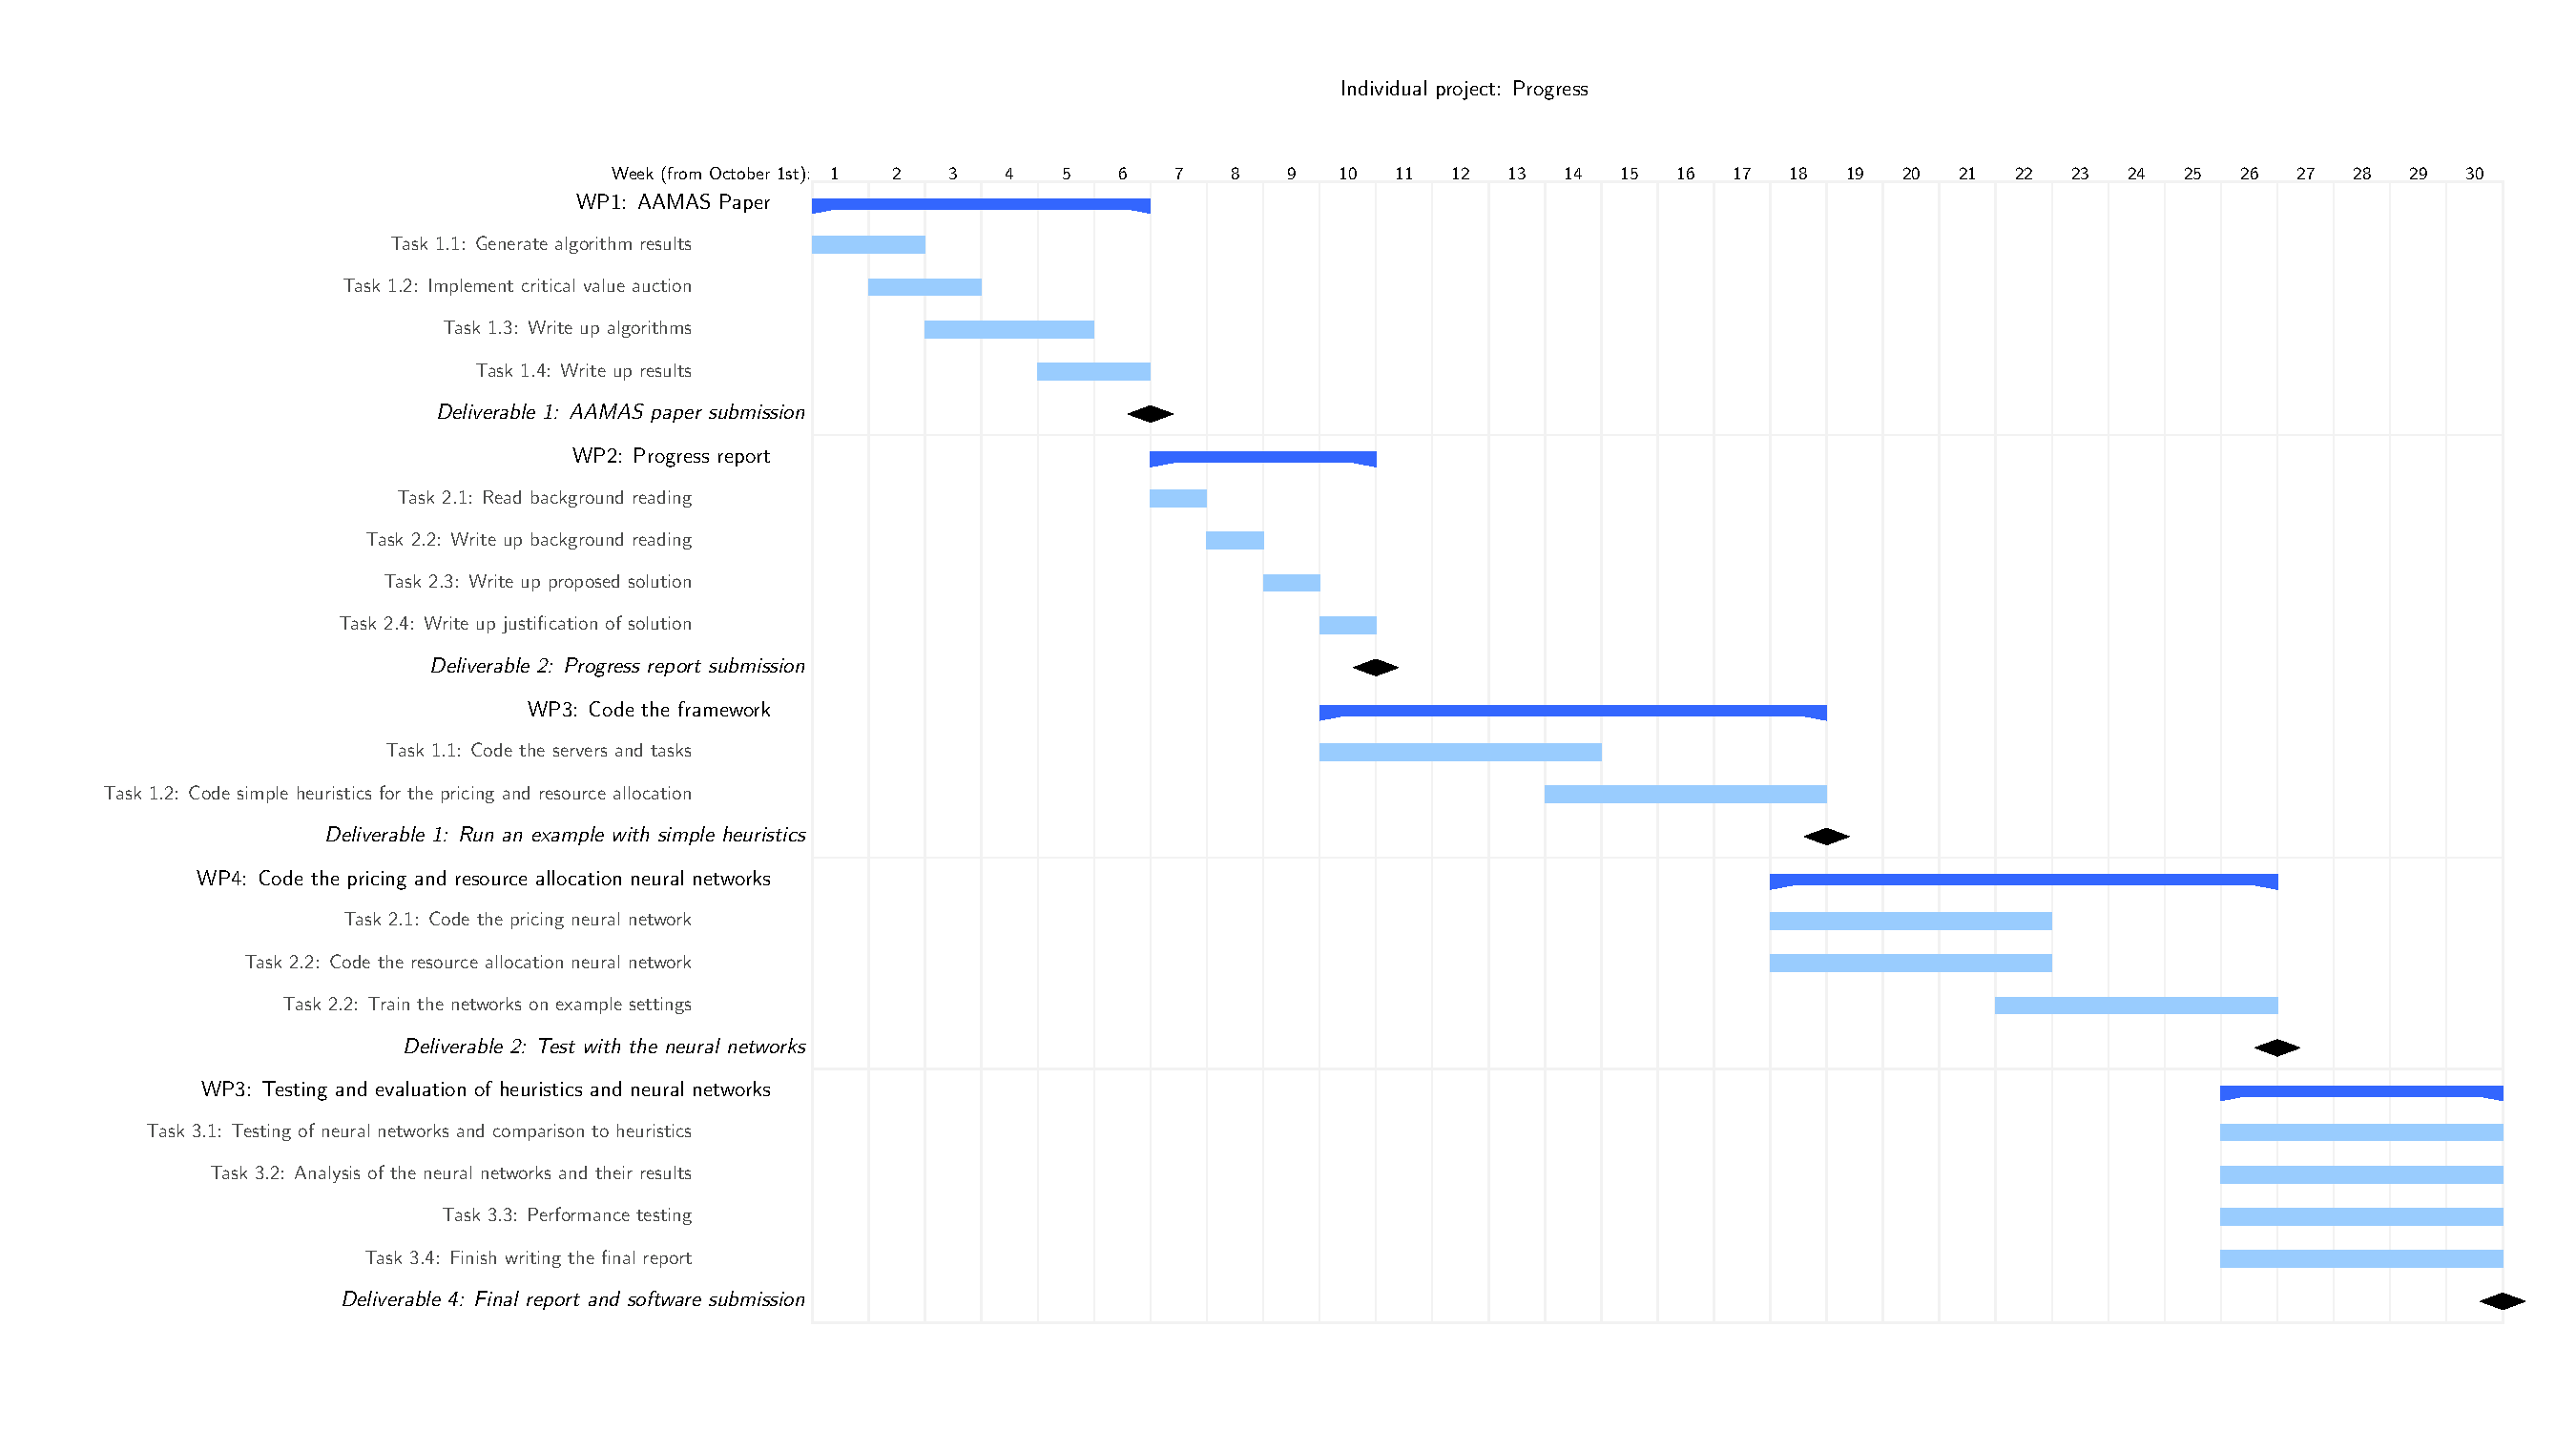
\includegraphics[width=13cm]{extra/expected_progress_grantt_chart.pdf}
    \caption{Expected Progress Grantt chart}
    \label{fig:expected-progress-grantt-chart}
\end{figure}

\begin{figure}[H]
    \centering
    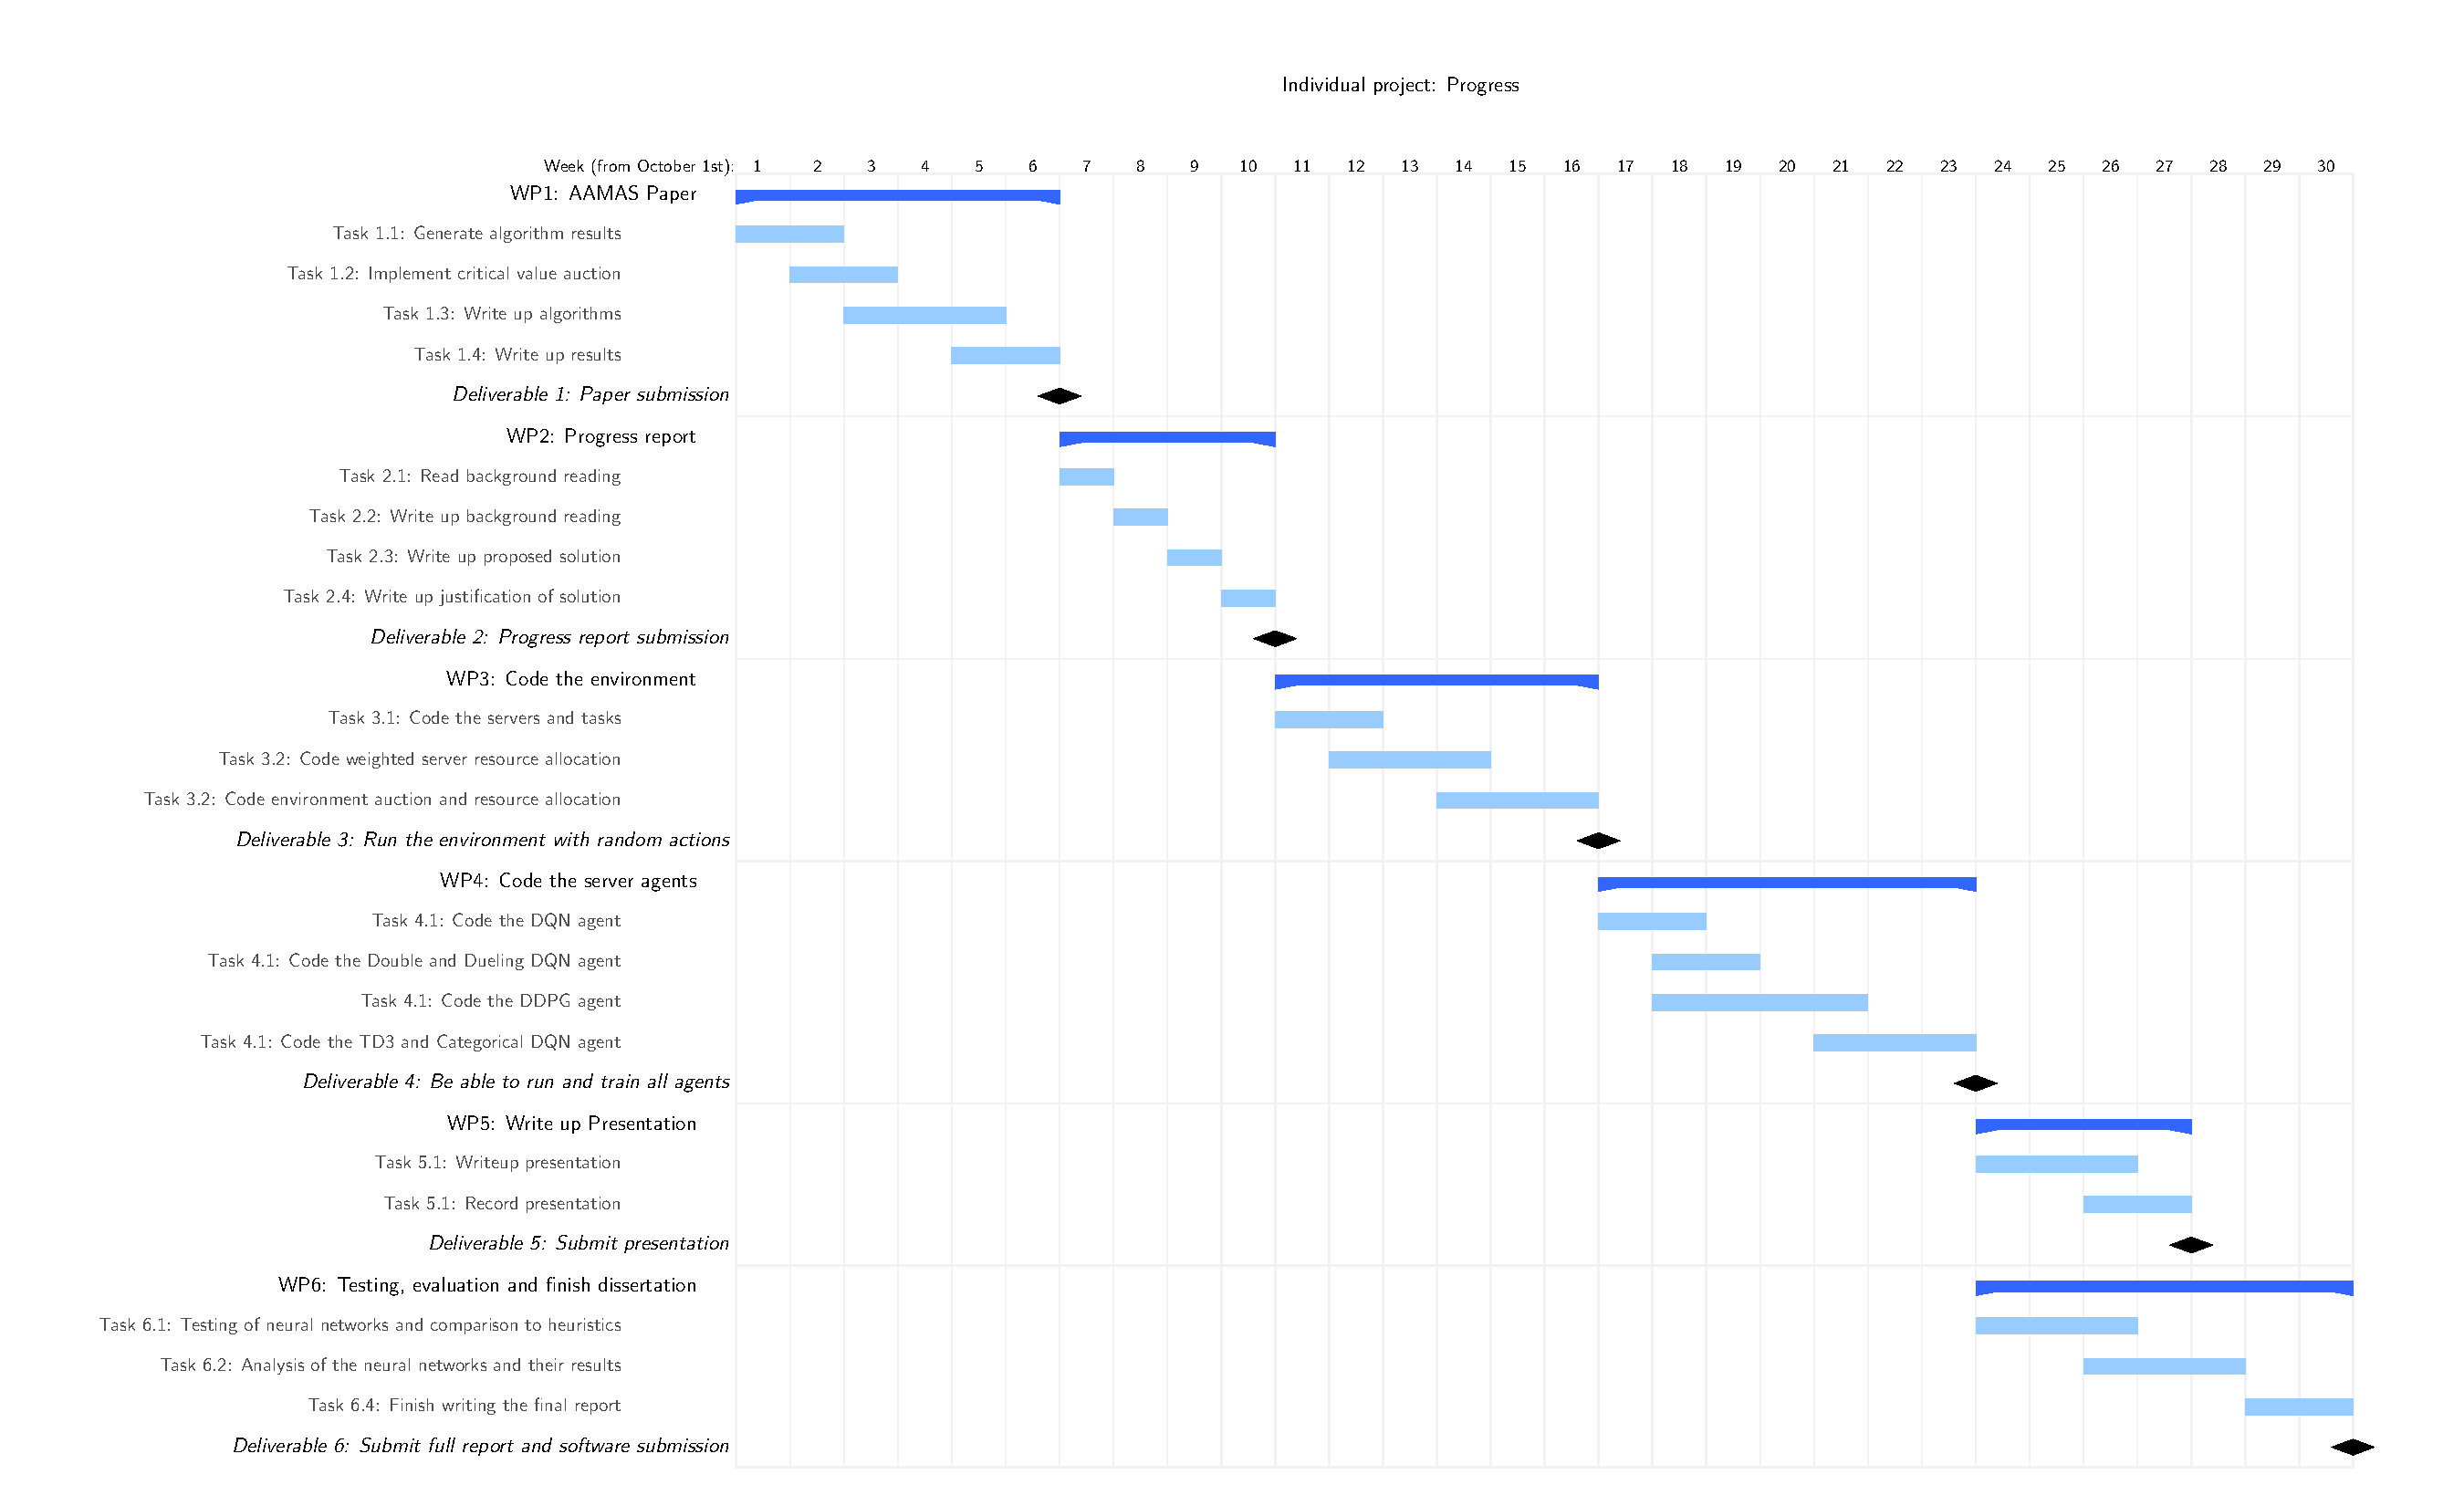
\includegraphics[width=14cm]{extra/progress_grantt_chart.pdf}
    \caption{Actual Progress Grantt chart}
    \label{fig:progress-grant-chart}
\end{figure}

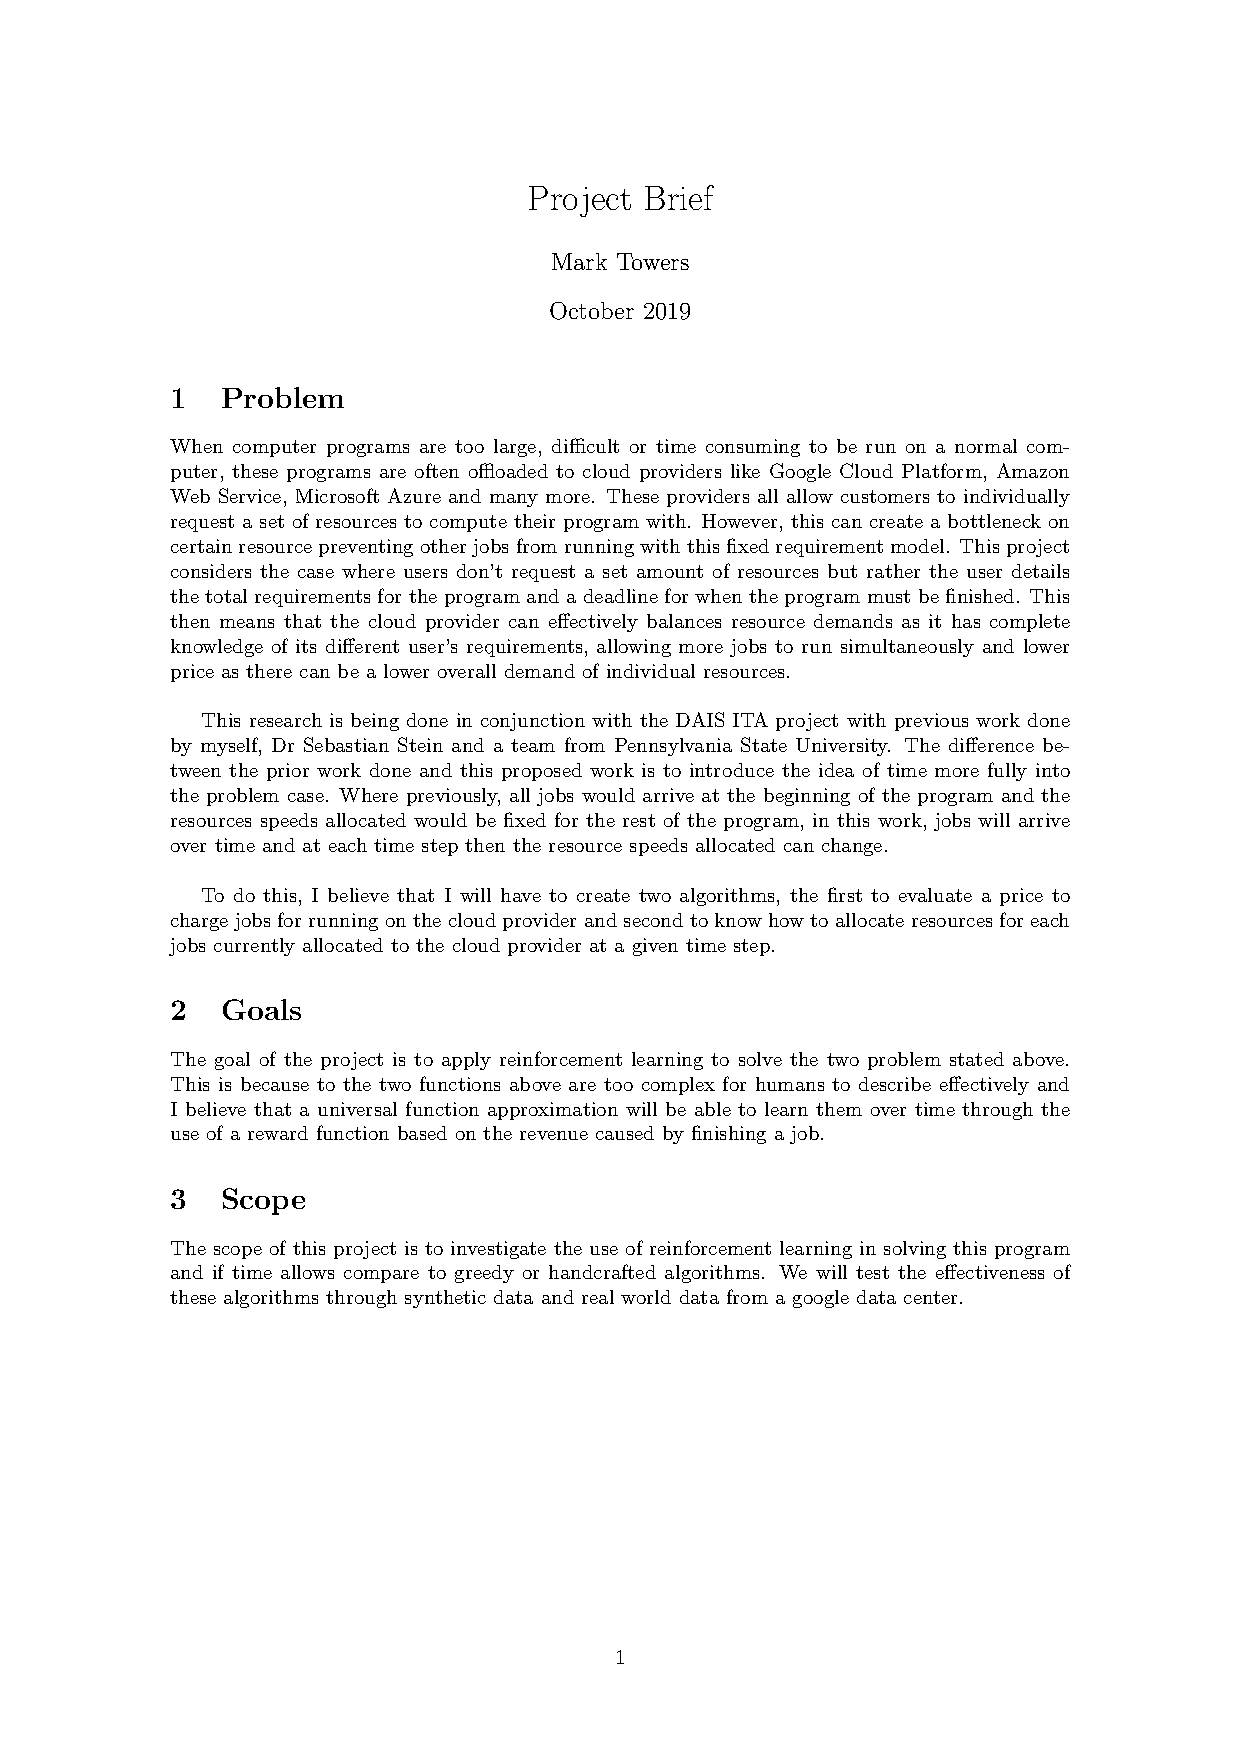
\includepdf[pages=-, offset=25mm -20mm]{extra/project_brief}

\subsection*{Word count}
% texcount -sum -inc chapters/1_introduction.tex chapters/2_background_lit.tex chapters/3_solution.tex chapters/4_implementation.tex chapters/5_evaluation.tex chapters/6_conclusion.tex -out=extra/wordcount.sum
\wordcount
